\documentclass[journal]{IEEEtran}
\usepackage{cite}
\usepackage{amsmath}
\usepackage{graphicx}
\usepackage[hidelinks]{hyperref}
\usepackage{cleveref}

\begin{document}

\title{Real-time Chord Recognition}
\author{Adam Belhouchat, Ashish Sareen}
\maketitle

\begin{abstract}
    Blahdy blah.
\end{abstract}
\begin{IEEEkeywords}
    Blah, blahdy, bloo
\end{IEEEkeywords}

\section{Introduction}
\subsection{History with References}
Automatic chord recognition (ACR) is the process of determining what chord is being played given an audio sample, labelling the audio sample over time with the appropriate chord \cite{stark}.
A chord here is defined as two or more notes being played at the same time or close together \cite{cho}.
Chord recognition has many applications, such as music segmentation or determining the similarity between two music samples \cite{lee}, but one of the most attractive applications is in automatic transcription.
Manual transcription can be tedious and difficult, and automatic chord recognition systems can help musicians work more quickly and more accurately \cite{mauch_thesis}.
Because of its wide range of applications, chord recognition has been the subject of much research in the past few decades, trying to improve the number of chords it can recognize and its accuracy through novel methods and approaches \cite{pauwels}.

One of the first ACR systems was developed by Takuya Fujishima in 1999 \cite{pauwels}.
He used the discrete Fourier transform (DFT) of a music sample to generate a pitch class profile, also known as chroma feature or chroma vector, which encodes the harmonic information of the sample over twelve different pitch classes.
The chroma feature is then compared the templates, one for each of 27 different chords, and the closest match is chosen as the chord label in a process called pattern matching \cite{fujishima}.

Since then, chord recognition has evolved greatly.
Pattern matching is simple and effective, but it is not the most accurate \cite{jiang}.
Some researchers have found great success using hidden Markov models (HMMs) rather than template matching to perform ACR \cite{sheh}, and others have explored the use of deep learning and neural networks both to detect chords \cite{boulanger} and to extract features from the audio sample \cite{korzeniowski}.
However, both HMMs and deep learning require a significant amount of training data, and good training data may be difficult to come by.
Manual transcription is prone to errors due to human subjectivity \cite{pauwels} and as mentioned before, it can be time consuming.
Nevertheless, these approaches do show significant accuracy improvements over pattern matching \cite{jiang, boulanger}.
Each of these approaches has its pros and cons, and which one is most fitting depends on the specific application.


\subsection{Global Constraints}

\section{Motivation}
One shortcoming of many modern chord recognition systems is the vast amount of data required to train these systems \cite{pauwels}.
As mentioned earlier, large datasets of accurately transcribed music are not easy to find, so we wanted to develop a system that would work without training.
Additionally, these data-driven approaches are opaque and it is difficult to understand how they determine the chords in an audio sample \cite{pauwels}.
Part of our motivation for pursuing this project was to increase our skills in real-time digital signal processing and to understand how automatic chord recognition works.
Throwing data at a neural network until it works does not help us understand chord recognition.

Another shortcoming of HMMs and neural networks is they are often more computationally expensive than pattern matching \cite{stark}.
They work well when a music sample has been prerecorded and is later fed into the system, but they are not fast enough to perform chord recognition and transcription in real-time.
We wanted to make a chord recognition system that would record musical chords and transcribe them in real-time, so we needed to approach our system differently from most modern systems.

Lastly, as mentioned earlier, we chose this project to learn more about real-time digital signal processing (DSP) and to gain more experiences with different applications of it.
Chord recognition requires many DSP techniques, including sampling a signal, processing it to extract features, performing some evaluation on those features, and then returning the results of that evaluation to the user \cite{fujishima}.
This project would give us valuable experience with all the important elements of DSP with the added constraint of performing it in real-time.
This required us to perform memory management and pay close attention to our code to make sure all functions were optimized, which are valuable skills for embedded software development.

\section{Approach}
\subsection{Team Organization}

\subsection{Plan and Implementation}

\subsection{Standard}
The most common features used in pattern matching and HMM chord recognition systems are chroma features \cite{cho_chroma}.
First introduced into chord recognition by Fujishima, basic chroma features are calculated by summing the DFT of the music signal over certain frequency bins \cite{fujishima}.
Each chroma vector has twelve elements corresponding to the twelve pitch classes that the frequency bins are mapped to, and the distribution of energy across the twelve pitch classes determines which chord it corresponds to \cite{jiang}.
Because of how ubiquitous chroma features are in chord recognition, we chose to use them as our features for chord recognition.

To actually determine what chord the chroma features corresponds to, we use pattern matching, which is one of the most common methods of determining chords \cite{cho_chroma}.
In particular, we use binary pattern matching, where each chord has a corresponding template which is a specific arrangement of zeros and ones.
The tones present in the ideal chord are one, while all the other tones are zero \cite{cho_chroma}.
To find the matching template, many implementations look for the minimum Euclidean distance between a template and the chroma feature \cite{stark}, but other approaches such as finding the minimum angle between the two are also used \cite{jiang}.
We chose to go with this latter approach as it gave us slightly better accuracy.

\subsection{Theory}
The key mathematical elements of our chord recognition system are the low-pass filter, the chroma features, and pattern matching.
In this section, we will explain in detail the theory behind each of these steps.

The low-pass filter is generated using the bilinear transform, which converts a continuous transfer function to a discrete one.
To do so, the bilinear transform uses the approximate map
\begin{equation}
    s \to \frac{2}{T}\frac{1 - z^{-1}}{1 + z^{-1}}
    \label{eq:s_to_z}
\end{equation}
where T is the sampling period of the discrete signal.
We can then substitute this into the continuous transfer function $H_a(s)$ to get the discrete one $H_d(z)$ by 
\begin{equation}
    H_d(z) = H_a\!\left(\frac{2}{T}\frac{1 - z^{-1}}{1 + z^{-1}}\right)
    \label{eq:bilinear}
\end{equation}
Once we have $H_d(z)$, we can get the discrete time-domain equation by partial fractions and inverse Z-transform pairs.

We used a 6th order Butterworth low-pass filter with a cutoff frequency at 6000 Hz.
This cutoff frequency preserved most of the important harmonic information while still filtering out high-frequency noise, and the order gave a reasonably steep dropoff around the cutoff frequency without being computationally expensive.
The actual transfer function is too large and complex to show here, so we used a program to generate the time-domain filter function.
The frequency response is given in \Cref{fig:frequency_response}.

\begin{figure}[t]
    \centering
    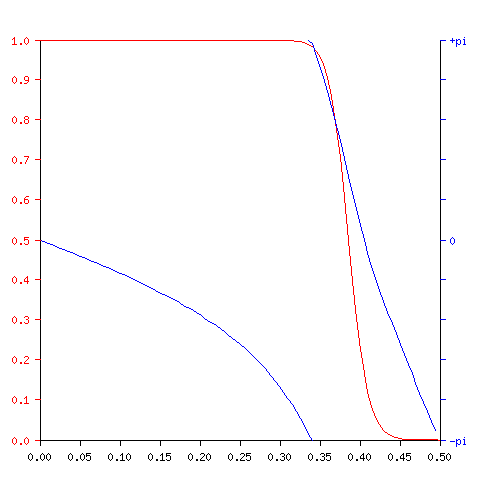
\includegraphics[width=\linewidth]{../Figures/frequency_response}
    \caption{Frequency response of the low-pass filter used in our chord recognition system.
    Courtesy of Tony Fisher at \url{https://www-users.cs.york.ac.uk/~fisher/mkfilter/}.}
    \label{fig:frequency_response}
\end{figure}

Chroma features are features that describe the pitch content of a sample of music \cite{jiang}. A chroma feature has 12 elements, one for each note in an octave from C through B. The value of one of these elements corresponds to the energy present in the music signal coming from that pitch. Because of this, it is straightforward to determine the chords in a piece of music by analyzing the chroma features.

The algorithm we use to generate chroma features comes from Stark and Plumbley’s paper \cite{stark}. The first step is to apply a Hamming window $w(n)$ to the signal $x(n)$, given by
\begin{equation}
    w(n) = 0.54 - 0.46\cos\!\left(\frac{2\pi n}{N - 1}\right)
    \label{eq:window}
\end{equation}
where $N$ is the size of the signal. Once we have the windowed signal $x_w(n) = x(n)w(n)$ we take the DFT,
\begin{equation}
    X(k) = \sum_{n = 0}^{N - 1}x_w(n)e^{-\frac{i2\pi kn}{N}}
    \label{eq:dft}
\end{equation}

From here, the original chroma feature algorithm would sum the squared magnitudes of the DFT over certain frequency bins to get the chroma values \cite{fujishima}. However, this may include unwanted energy like noise in the chroma features. To avoid this, Stark and Plumbley only consider the maximum amplitude in a given frequency bin, thus only taking into account the energy in the note we want.

First, we determine the frequencies to search over. We start with $f_{C3} = 130.81$ Hz, which is lower C. Then for $n = 0, 1, \ldots, 11$, we calculate
\begin{equation}
    f(n) = f_{C3}2^{(n / 12)}
    \label{eq:freq}
\end{equation}
which gives the 12 notes in an octave. We then do this for two octaves so we get all 24 notes in the two octaves from $f_{C3} = 130.81$ Hz to $f_{C5} = 523.25$ Hz. For each of the 12 elements of the chroma feature, we search through two octaves and within each octave search through two harmonics. This is because Stark and Plumbley have found that most instruments of interest use the lower register within this frequency range and to account for inharmonicities in real instruments \cite{stark}. The chroma feature is then given by
\begin{equation}
    c_n = \frac{1}{h}\sum_{\phi = 1}^2\sum_{h = 1}^2 \max_{k_0^{(n, \phi, h)} \leq k \leq k_1^{(n, \phi, h)}} X(k)
    \label{eq:chroma}
\end{equation}
where $c_n$ are the elements of the chroma vector $\mathbf{c}$, $n = 0, 1, \ldots, 11$, $\phi$ is the number of the octave, $h$ is the number of the harmonic, and 
\begin{equation*}
    k_0^{(n, \phi, h)} = k'^{(n, \phi, h)} - rh
\end{equation*}
\begin{equation*}
    k_1^{(n, \phi, h)} = k'^{(n, \phi, h)} + rh
\end{equation*}
where $r = 2$ is the number of bins to search over for each harmonic and 
\begin{equation*}
    k'^{(n, \phi, h)} = \text{round}\!\left(\frac{f(n)\phi h}{f_s / N}\right)
\end{equation*}
where $f_s$ is the sampling rate.

Lastly, we use pattern matching to match the chroma feature to the most fitting chord. Pattern matching involves the use of template vectors for each chord, such as $\mathbf{v}_C = (1, 0, 0, 0, 1, 0, 0, 1, 0, 0, 0, 0)$ for major C \cite{jiang}. We try to match the chroma vector to the closest template vector and from that get the corresponding chord. One simple method is to just find the Euclidean distance $||\mathbf{c} - \mathbf{v}||$ between the chroma vector and each of the template vectors and see which is the smallest. Another approach, which we use,  is to find the cosine similarity between two vectors, defined as 
\begin{equation}
    \text{cossim}(\mathbf{c}, \mathbf{v}) = \frac{\langle\mathbf{c}, \mathbf{v}\rangle}{||\mathbf{c}|| \cdot ||\mathbf{v}||}
    \label{eq:cossim}
\end{equation}
and choose the template vector with the maximum cosine similarity \cite{jiang}.

\subsection{Software/Hardware}

\subsection{Operation}

\subsubsection{How the System was Built}

\subsubsection{How to Use the System}

\section{Results}
\subsection{Description}
\subsection{Discussion}

\bibliographystyle{IEEEtran}
\bibliography{refs}

\end{document}